%%
% The BIThesis Template for Bachelor Graduation Thesis (School of Automation)
%
% 北京理工大学毕业设计开题报告 —— 使用 XeLaTeX 编译
%
% Copyright 2021 Charlie Li built upon Spencer Woo
%  
%
% This work may be distributed and/or modified under the
% conditions of the LaTeX Project Public License, either version 1.3
% of this license or (at your option) any later version.
% The latest version of this license is in
%   http://www.latex-project.org/lppl.txt
% and version 1.3 or later is part of all distributions of LaTeX
% version 2005/12/01 or later.
%
% This work has the LPPL maintenance status `maintained'.
%
% The Current Maintainer of this work is Spencer Woo.
%
% This work consists of the files main.tex, misc/cover.tex and
% the external PDF misc/reviewTable.pdf
%
% Compile with: xelatex -> bibTeX -> xelatex -> xelatex

\documentclass[UTF8,AutoFakeBold,AutoFakeSlant,zihao=-4]{ctexart}
\usepackage[a4paper,left=3cm,right=2.4cm,top=2.6cm,bottom=2.38cm,includeheadfoot]{geometry}
\usepackage{fontspec}
\usepackage{setspace}
\usepackage{graphicx}
\usepackage{fancyhdr}
\usepackage{pdfpages}
\usepackage{setspace}
\usepackage{booktabs}
\usepackage{multirow}
\usepackage{caption}
\usepackage[normalem]{ulem}

% 参考文献引用文件 refs.bib
\bibliographystyle{abbrv} 
% 去掉Reference小标题,采用section形式 
\usepackage{etoolbox}
\patchcmd{\thebibliography}{\section*{\refname}}{}{}{}
\newcommand{\upcite}[1]{\textsuperscript{\cite{#1}}}  %自定义新命令\upcite, 使参考文献引用以上标出现

% 下方填入开题报告的基本信息
\newcommand{\thesistitle}{双轴旋转惯性导航系统自标定技术研究}
\newcommand{\deptName}{自动化学院}
\newcommand{\majorName}{自动化国际班}
\newcommand{\className}{06911701}
\newcommand{\yourName}{张叁}
\newcommand{\mentorName}{李嗣}
\newcommand{\offCampusMentorName}{王舞}

% 定义 caption 字体为楷体
\DeclareCaptionFont{kaiticaption}{\kaishu \normalsize}

% 设置图片的 caption 格式
\renewcommand{\thefigure}{\thesection-\arabic{figure}}
\captionsetup[figure]{font=small,labelsep=space,skip=10bp,labelfont=bf,font=kaiticaption}

% 设置表格的 caption 格式
\renewcommand{\thetable}{\thesection-\arabic{table}}
\captionsetup[table]{font=small,labelsep=space,skip=10bp,labelfont=bf,font=kaiticaption}

% 定义一个概念
\newtheorem{definition}{概念}[section]

% 输出大写数字日期
\CTEXoptions[today=big]

% 将西文字体设置为 Times New Roman
\setromanfont{Times New Roman}

%% 将中文楷体设置为 SIMKAI.TTF(如果需要)
% \setCJKfamilyfont{zhkai}{[SIMKAI.TTF]}
% \newcommand*{\kaiti}{\CJKfamily{zhkai}}

% 设置文档标题深度
\setcounter{tocdepth}{3}
\setcounter{secnumdepth}{3}

%%
% 设置一级标题、二级标题格式
% 一级标题:小三,宋体,加粗,段前段后各半行
\ctexset{section={
  format={\raggedright \bfseries \songti \zihao{-3}},
  number = \chinese{section},
  beforeskip = 24bp plus 1ex minus .2ex,
  afterskip = 24bp plus .2ex,
  fixskip = true,
  name = {,、}
  }
}
% 二级标题:小四,宋体,加粗,段前段后各半行
\ctexset{subsection={
  format = {\bfseries \songti \raggedright \zihao{4}},
  beforeskip =24bp plus 1ex minus .2ex,
  afterskip = 24bp plus .2ex,
  fixskip = true,
  }
}

%%
% 文档开始
\begin{document}

% 报告封面
%%
% The BIThesis Template for Bachelor Graduation Thesis
%
% 北京理工大学毕业设计开题报告 —— 使用 XeLaTeX 编译
%
% Copyright 2020 Spencer Woo
%
% This work may be distributed and/or modified under the
% conditions of the LaTeX Project Public License, either version 1.3
% of this license or (at your option) any later version.
% The latest version of this license is in
%   http://www.latex-project.org/lppl.txt
% and version 1.3 or later is part of all distributions of LaTeX
% version 2005/12/01 or later.
%
% This work has the LPPL maintenance status `maintained'.
%
% The Current Maintainer of this work is Spencer Woo.
%
% This work consists of the files main.tex, misc/cover.tex and
% the external PDF misc/reviewTable.pdf


\begin{titlepage}
	\vspace*{5mm}
	\centering
	\hspace{-6mm}
\includegraphics[width=0.45\linewidth]{misc/logo}
	
	\vspace{3mm}
	
	\hspace{-6mm}\heiti\fontsize{24pt}{24pt}\selectfont{\textbf{毕业设计(论文)\\开题报告}}
	
	\vspace{23mm}
	
	\flushleft
	\begin{spacing}{2.2}
		\hspace{12mm}\songti \fontsize{16pt}{16pt} \selectfont{\textbf{毕业设计(论文)题目:} \begin{minipage}[t]{80mm} \CJKunderline*{\thesistitle \hfill }
		\end{minipage}}
		\vspace{30mm}
		
		\hspace{46mm}\songti\fontsize{16pt}{16pt}\selectfont{\textbf{学\hspace{11mm}院:}\underline{\makebox[51mm][c]{\deptName}}}
		
		\hspace{46mm}\songti\fontsize{16pt}{16pt}\selectfont{\textbf{专\hspace{11mm}业:}\underline{\makebox[51mm][c]{\majorName}}}
		
		\hspace{46mm}\songti\fontsize{16pt}{16pt}\selectfont{\textbf{班\hspace{11mm}级:}\underline{\makebox[51mm][c]{\className}}}
		
		\hspace{46mm}\songti\fontsize{16pt}{16pt}\selectfont{\textbf{姓\hspace{11mm}名:}\underline{\makebox[51mm][c]{\yourName}}}
		
		\hspace{46mm}\songti\fontsize{16pt}{16pt}\selectfont{\textbf{指导教师:}\underline{\makebox[51mm][c]{\mentorName}}}
		
		% 没有的话可以注释掉
		\hspace{46mm}\songti\fontsize{16pt}{16pt}\selectfont{\textbf{校外指导教师:}\underline{\makebox[40mm][c]{\offCampusMentorName}}}
	\end{spacing}

\end{titlepage}
 

% 评审表
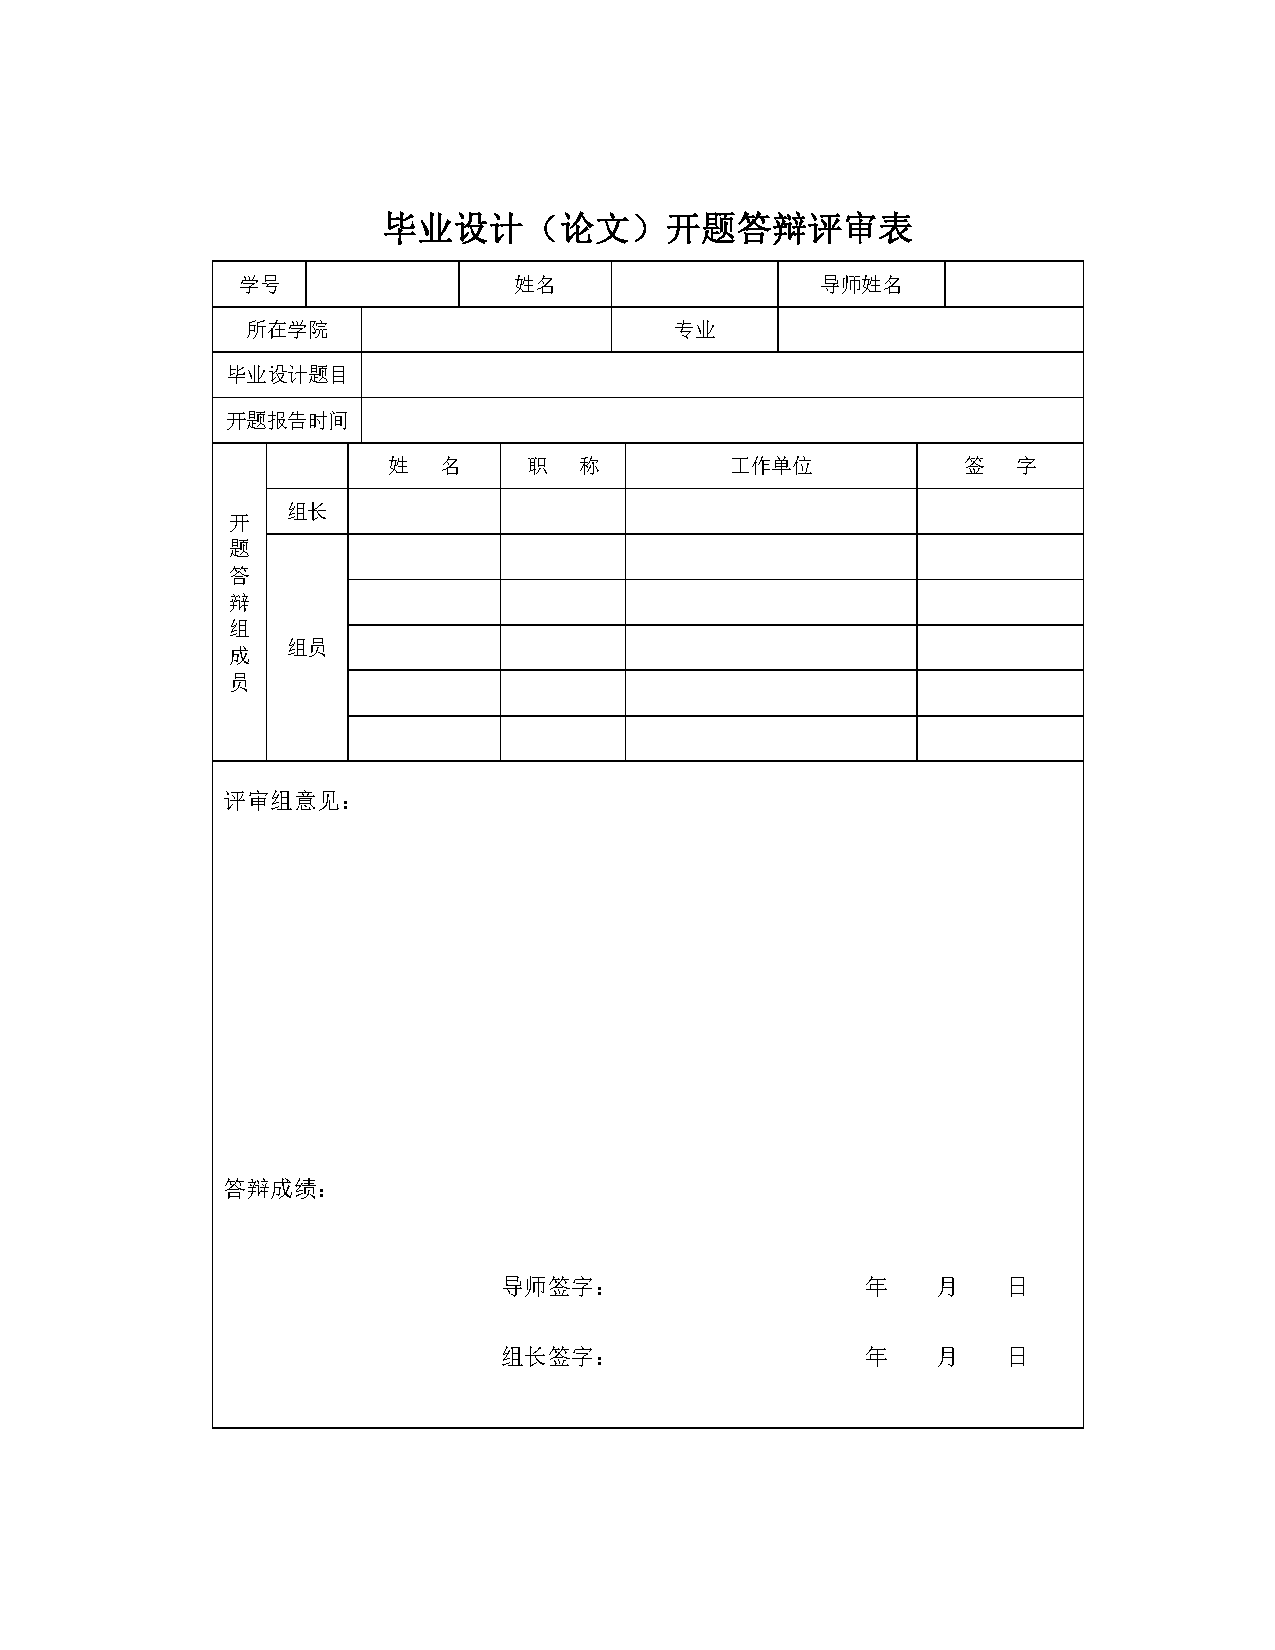
\includepdf[pages=-,scale=1.2]{misc/reviewTableBlank.pdf}

%%
% 正文开始
\pagestyle{fancy}
% 正文从第一页开始计算页码
\setcounter{page}{1}
% 页眉和页脚(页码)的格式设定
\fancyhf{}

%\fancyhead[R]{\fontsize{10.5pt}{10.5pt}\selectfont{北京理工大学本科生毕业设计(论文)开题报告}}
\fancyfoot[C]{\fontsize{9pt}{9pt}\selectfont{\thepage}}
% 去掉header & footer的线
\renewcommand{\headrulewidth}{0pt}
\renewcommand{\footrulewidth}{0pt}

% 正文 22 磅的行距,段前段后间距为 0
\setlength{\parskip}{0em}
\renewcommand{\baselinestretch}{1.53}
% 正文首行悬挂 1.02cm
\setlength{\parindent}{1.02cm}

% 内容开始
\section{毕业设计(论文)任务书}
开题报告总长度约 5 至 6 页,本部分重点介绍毕业设计选题的主要内容 \upcite{LeCun2010},宋体,小三,段落前后 0.5 行。

\subsection{题目内容}
\subsection{任务要求}
\noindent 注意事项:
\begin{enumerate}
	\item 小标题字号:四,行间距:固定值22磅,
	\item 内容字号:小四,行间距:固定值22磅,首行缩进2个字符  
	\item 所有部分  中文:宋体;英文:TIMES NEW ROMAN字体
\end{enumerate}

\section{选题的背景和意义}
\subsection{研究背景与意义}
本部分重点关注毕业设计的主要任务,宋体,四号,段落前后 0.5 行。

\subsection{国内外研究现状和发展趋势}
此部分要分析任务书,并给出初步方案,要体现出复杂系统的概念,约写 2 至 3 页。





\section{研究方案}
\subsection{}
\subsection{}

\section{实施技术方案所需要的条件}
\subsection{}
\subsection{}

\section{预期成果}

\section{时间安排}
大致的课题计划进度如下表 \ref{tab:progress} 所示。


% 调整时间表的arraystretch
\renewcommand*\arraystretch{2.4} 
\begin{table}[!ht]
  \centering
  \caption{毕业设计计划进度表}
  \label{tab:progress}
  \begin{tabular}{@{}cc@{}}
    \toprule
    时间 & 计划完成工作       \\ \midrule
    3.1—3.8 & 撰写开题报告,完成开题答辩 \\\hline
    & \\\hline
    & \\\hline
    6.3—6.11 & 完成最终答辩\\\bottomrule
  \end{tabular}
\end{table}


注意:下文的参考文献应包含近 5 年内文献,经典文献除外。

\section{参考文献}
% 将原来的biber编译方式改为bibTeX
\bibliography{ref}

\end{document}
